\documentclass{beamer}
\usepackage{lsfolien}
\usepackage[main=english,ngerman]{babel}
\usepackage[utf8]{inputenc}

\myfootline{System Modelling and Semantic Web -- Winter Term 2021}{Hans-Gert
  Gräbe}

\newcommand{\ueberschrift}[1]{\begin{center}\bf #1\end{center}}

\title{Modelling Sustainable Systems\\ and Semantic Web\\[6pt]
  Systemic Structures and Action Spaces
  \vskip1em}

\subtitle{Lecture in the Module 10-202-2309\\ for Master Computer Science}

\author{Prof. Dr. Hans-Gert Gräbe\\
\url{http://www.informatik.uni-leipzig.de/~graebe}}

\date{November 2021}
\begin{document}

{\setbeamertemplate{footline}{}
\begin{frame}
  \titlepage
\end{frame}}

\begin{frame}{Systemic Structures}

Systemic thinking means grouping closely interrelated processes into
\textbf{systemic units}.

Such units as components are characterised by their eigentimes and eigenspaces
in which stable, externally visible structures (limit cycles) reproduce
themselves.

Combining such components into a new system means coupling these repetitive
processes, usually resulting in systems whose characteristic eigentimes are
common multiples of the eigentimes of the components.

\end{frame}

\begin{frame}{Systemic Structures}
Of particular interest is the context in which fast-moving components are
embedded in a slow-moving system. In this case, two clearly different
dimensions of reduction to "essentials" arise: The external context can be
considered largely static in the analysis of the components, while in the
analysis of the external context, the behaviour of the components can be
reduced to a statistical mean in which "chaotic noise" averages out and thus
becomes irrelevant for the modelling at the level of the slow-moving system.

\end{frame}

\begin{frame}{Systemic Structures}

  \emph{Example:} A technical system with two components -- the car body
  department of a car manufacturer with press subdepartment and coloring
  subdepartment.
    
  \begin{minipage}{.42\textwidth}\centering\vspace*{2em}
    \begin{tikzpicture}[line width=1pt]
        \node[draw,text width=3em, align=center] [circle] (A0) {CBD};
        \node[draw,below left=of A0, node distance=2em] [circle] (A1) {PS};
        \node[draw,below right=of A0, node distance=2em] [circle] (A2) {CS};
        \draw[-,dashed] (A0)--(A1) ;
        \draw[-,dashed] (A0)--(A2) ;
    \end{tikzpicture}\\[2em] Structural Organisation
  \end{minipage}\hfill
  \begin{minipage}{.55\textwidth}\centering
    \begin{tikzpicture}[line width=1pt,scale=.7,transform shape]
    \node[draw,text width=3em, align=center] [circle] (A0) {CBD};
    \node[draw,text width=2cm, align=center, above left=of A0] [rectangle] (I)
         {Input\\Metal Sheet}; 
    \node[draw,text width=2cm, align=center, above right=of A0] [rectangle] (O)
         {Output\\Finished Car Body}; 
    \node[draw,below left=of A0, node distance=2em] [circle] (A1) {PS};
    \node[draw,below right=of A0, node distance=2em] [circle] (A2) {CS};
    \draw[->] (I)--(A0) ;
    \draw[->] (A0)--(O) ;
    \draw[->] (A0) to[bend right] (A1) ;
    \draw[->] (A1) to[bend right] (A0) ;
    \draw[->] (A0) to[bend right] (A2) ;
    \draw[->] (A2) to[bend right] (A0) ;
    \end{tikzpicture}\\[2em] Workflow Organisation
  \end{minipage}
\end{frame}

\begin{frame}{Systemic Structures}

Spatial structures can be composed immersively, temporal structures can be
projected submersively onto different time scales through Fourier
transformations.

The temporal structures considered determine the reduction dimension and thus
select the processes that are "essential" for the systemic context; the
spatial structure of the flows of energy, matter and information moved in the
process determines the spatial extent of the systemic context.

This does not only apply to models of technical or business systems but ...
\end{frame}

\begin{frame}{Systemic Structures}

  ... typically structures also models of socio-economic systems ...
  \begin{center}
    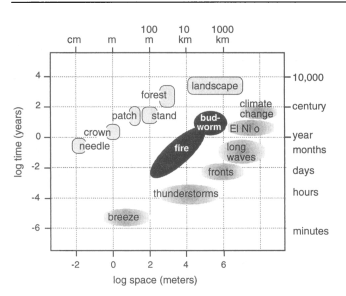
\includegraphics[width=.6\textwidth]{Bilder/Holling-1.png}

    Diagram from (Holling 2001)
  \end{center}
\end{frame}

\begin{frame}{Systemic Structures}
  \begin{center}

    ... of socio-cultural systems ... 
    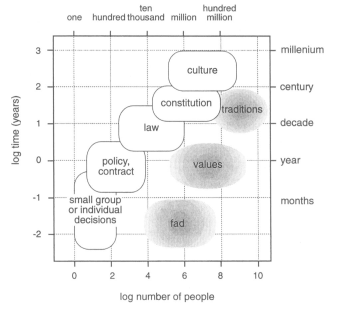
\includegraphics[width=.6\textwidth]{Bilder/Holling-2.png}

    Diagram from (Holling 2001)
  \end{center}
\end{frame}

\begin{frame}{Systemic Structures}

  ... and also of "natural" systems.
  \begin{center}
    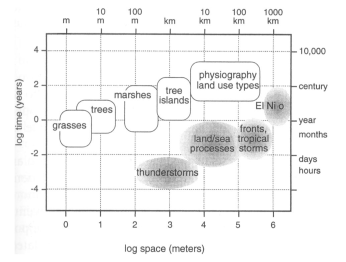
\includegraphics[width=.7\textwidth]{Bilder/Holling-3.png}

    Diagram from (Holling 2001)
  \end{center}
\end{frame}

\begin{frame}{Development of Systemic Structures}

  \emph{Example:} The press department is modernised, industrial robots are
  being used.  How does that affect the other components of the systems?

  What scenarios are conceivable?

\end{frame}

\begin{frame}{Development of Systemic Structures}

  \begin{minipage}{.4\textwidth}
    Which typical scenarios are to be distinguished for systems that develop
    along an attractor?
  \end{minipage}\hfill
  \begin{minipage}{.55\textwidth}\centering
    \begin{tikzpicture}[scale=.55,line width=1pt,transform shape]
      \node (A0) at (0,10) {};
    \node (A4) at (3,8.5) {};
    \node (A1) at (5,7) {};
    \node (A1a) at (7,6.5) {};
    \node (A2) at (0,5) {};
    \node (A3) at (7,0) {};
    \node (A5) at (6.5,4) {};
    \node (A6) at (6,.5) {};
    \draw plot [smooth] coordinates {(A0) (A4) (A1) (A2) (A6) (A3)};
    \node[draw=red] at (4.2,9.2) [rectangle] {$r$ Phase};
    \draw[<->] (2.3,8.1) -- (3.1,7.7) ;
    \node[draw=red] at (6.2,7.5) [rectangle] {$K$ Phase};
    \draw[<->] (4.7,6.5) -- (5.5,6.5) ;
    \node[draw=red] at (8.2,6.5) [rectangle] {$\Omega$ Phase};
    \draw[->] (6.7,5.9) -- (6.6,5.3) ;
    \node[draw=red] at (8,3.8) [rectangle] {$\alpha$ Phase};
    \draw[->] (6.2,3.4) -- (6.1,2.8) ;
    \draw[<->] (5.2,.3) -- (6.2,-.2) ;
    \draw[fill=green] (A4) circle (6pt) ;
    \draw[->,dashed] plot [smooth] coordinates {(A1) (A1a) (A5) (A6)};
    \draw[fill=green] (A1) circle (6pt) ;
    \draw[fill=green] (A1a) circle (6pt) ;
    \draw[fill=green] (A5) circle (6pt) ;
    \draw[fill=green] (A6) circle (6pt) ;
    \node[draw=red,fill=white] at (7.5,0.9) [rectangle] {neue $r$-Phase};
  \end{tikzpicture}
  \end{minipage}
\end{frame}

\begin{frame}{Development of Systemic Structures}
  \begin{center}
    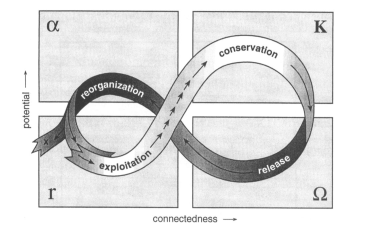
\includegraphics[width=.85\textwidth]{Bilder/Holling-4.png}
  \end{center}
\end{frame}

\begin{frame}{Development of Systemic Structures}
  \begin{center}
    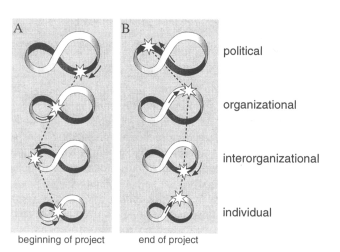
\includegraphics[width=.85\textwidth]{Bilder/Holling-5.png}
  \end{center}
\end{frame}

\begin{frame}{Action Spaces}

This structuring of the world, however, is a view of the structures
\textbf{from the outside}.

Even more, we have seen that the \emph{decomposability} into parts associated
with a structural view hides essential emergence phenomena and thus stands in
dialectical contradiction to the \emph{indecomposability} in the process view
-- a system can only be operated in an assembled state.

From the \textbf{internal perspective} of a system, processes can nevertheless
be analysed more precisely in a local environment. This is also the basis of
the \textbf{TRIZ concept of the operative zone}.

\end{frame}

\begin{frame}{Action Spaces}
Such a "view from within" shapes our perception of the world around us.
Practical experience is gained in \textbf{local contexts}, and
contextualisations always limit the meaning spaces of our generalisations.

\begin{block}{}
  We call such a view on a system from inside an \textbf{action space}.
\end{block}

Oxford Reference:
\begin{quote}
  It is the area in which individuals move and make decisions about her or
  his life.
\end{quote}

This definition is too narrow for a concept of cooperate action. 

\end{frame}

\begin{frame}{World and Reality}

  \begin{minipage}{.4\textwidth}\centering
    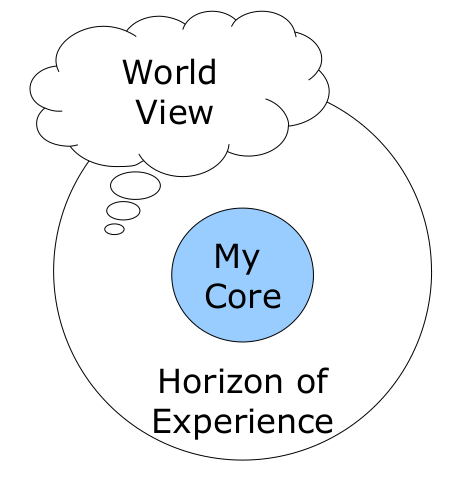
\includegraphics[width=\textwidth]{Bilder/DI-1.png}
  \end{minipage}\hfill
  \begin{minipage}{.55\textwidth}
    \ueberschrift{Private and Cooperative Action}
    \begin{itemize}
    \item Art of living versus dealing with a structured world in a structured
      way
    \item Unpredictability versus predictability
    \item Constructability of "world“
    \item Me as a constructor
    \item (My) imagination and reality
    \end{itemize}
  \end{minipage}

\end{frame}
\begin{frame}{World and Reality}\centering
    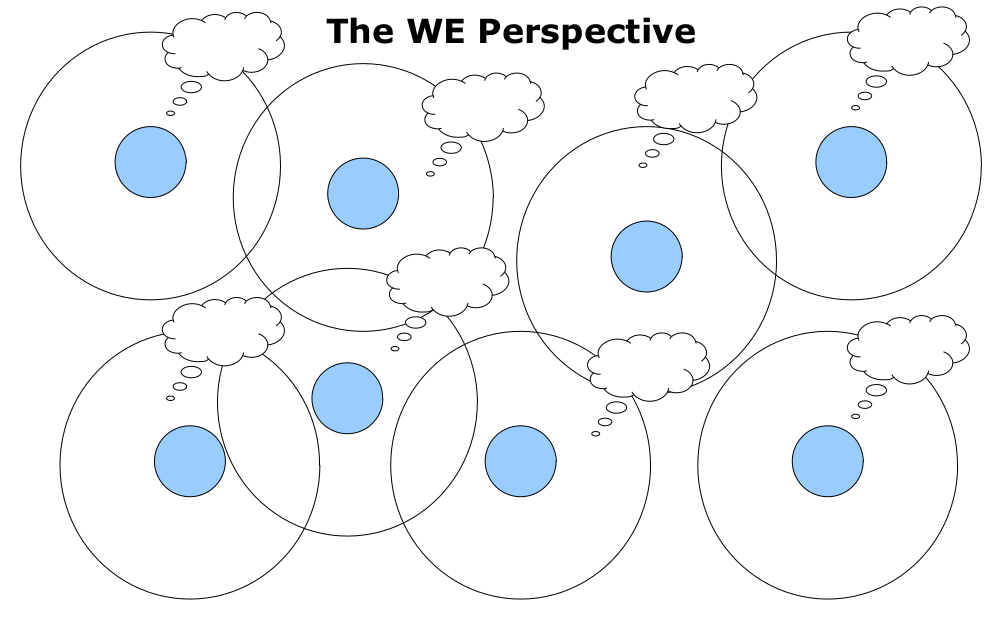
\includegraphics[width=.9\textwidth]{Bilder/DI-2.png}
\end{frame}
\begin{frame}{World and Reality}\centering
    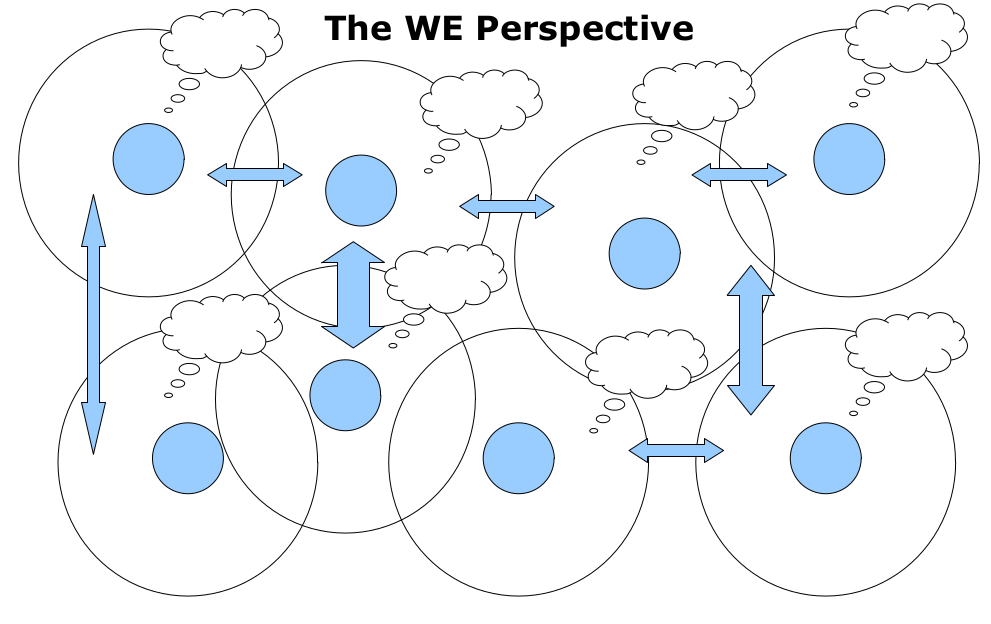
\includegraphics[width=.9\textwidth]{Bilder/DI-3.png}
\end{frame}
\begin{frame}{World and Reality. Starting Point}
  \begin{itemize}
  \item Forms of description (plural) and reality.
  \item Contradictoriness of the world (as reality perceived by us)
  \item Differences in the concept of \emph{contradiction} in forms of
    description and forms of actions
  \item Descriptions and contextualisations
    \begin{itemize}
    \item Creativity and conceptualisation
    \item Concepts are a form of cooperative practices of people and thus
      themselves are to be \emph{contextualised in a concrete-historical way}.
    \end{itemize}
  \item Term \emph{World View} for the complex context of the model-like
    reference \emph{in the model} to reality.
  \end{itemize}
  \begin{block}{World and Reality}
    \emph{World} is \emph{reality for us} and thus \emph{reality in the
      process of conceptual comprehension}.
  \end{block}
\end{frame}
\begin{frame}{World and Reality. What is Data?}
How objective are these world views? Do we all live in our own echo chambers
and filter bubbles?

\begin{center}  \LARGE\bf
  \vfill What is Data?\\[1em] What is objective Data? \vfill  
\end{center}

\end{frame}
\begin{frame}{World and Reality. What is Data?}
  \begin{itemize}
  \item Data as a specific form of description.
  \item Capturing data always means choosing what \emph{not} to capture.
  \item Data as a link between world and reality.
  \item But what then is \emph{objective} data?
    \begin{itemize}
    \item Specific reflex of a positivistic understanding of science.
    \item Use and misuse: Such an understanding (of science) is an important
      cultural achievement of humankind, which, however, also has to be
      \emph{contextualised in concrete-historical terms}.
    \end{itemize}
  \item Thus data is also a form of cooperative practices of people.
  \end{itemize}
\end{frame}
\end{document}
